%!TEX root = gutter+stars.tex
\chapter{Introduction}
\label{the introduction}

Despite common belief, software engineers do not spend most time writing code. An approximate 50--90\% of development time is spent on code navigation and understanding \cite{Abra04a,Lato06a,Ko07a}. This may include reading of local source code and documentation, searching the internet for tutorials and code examples, but also seeking help of other developers. 

User studies have found that software engineers use at least four kinds of cognitive clues for \codenavigation: 
	lexical clues, 
	social clues, 
	episodic clues 
	and spatial clues 
	\cite{Lato06a,Ko07a,Sill06a,Frit10a,Kuhn10x}.
%
Examples of code orientation by these clues are: 
	searching for an identifier name (lexical clue),
	contacting a coworker with known expertise (social clue), 
	referring to a design decision that was made years ago (episodic clue), or 
	navigating to the location of a piece of code within a source text file (spatial clue). 

%Tool support for \codenavigation, however, is typically limited to keyword-based text file processing and hyperlinking of code elements. 

In our research, we are interested in how to support software engineers when they are facing technical questions that involve code navigation and code understanding. We investigated how software engineers find answers to technical questions in order to learn about their \codenavigation strategies (\autoref{the chapter on the MSR user study}). 
We found that the way towards an answer is typically split into two parts. In a first part, developers aim to turn their fuzzy initial clue into a concrete textual clue, for example by running a series of web searches and inspecting the results. Developers particularly struggle to resolve social, episodic and spatial clues during the first part. In a second part, they use that newly found textual clue to query resources on the internet or in local documentation. This two-step procedure might be an artifact of current tool limitations, that is developers aim to find a lexical clue first because other clues are harder to follow up, or it might be a general problem-solution strategy. In either case, developers need better tool support to follow up non-textual clues such as social, episodic and spatial clues.

Among the code orientation strategies used by developers, spatial clues stand out for not having a first-class representation in the ecosystem of source code. 
%Textual clues have a representation in identifiers found in source code or to terms used in comments and documentation. Social clues are connected to coworkers and experts from a developer's network. Episodic clues are often related to events that have been recorded in the version control system and in mailing list archives. 
Spatial clues typically lack a first-class counterpart in source code since software systems do not have an inherent spatial extent. Nevertheless, we found that developers do refer to source code by \adhoc spatial properties, such as clues regarding the position of a code artifact on-screen or within a source text file. 
%
Given the potential of spatial clues for code navigation, we investigated how to best represent software systems using spatial visualizatons. 

In this dissertation we introduce \emph{Software Cartography}, a novel cartographic visualization of software systems that enables code orientation by on-screen spatial clues (\autoref{the chapter on codemap}). The \emph{software map} visualizations created by our approach offer a spatial representation of software systems based on lexical information found in the system's source code. Software maps are stable over time and can be used by individual developers as well as shared by a team. 

We implemented a prototype tool and evaluated it in a qualitative user study. We found that software maps are most helpful to explore search results and call hierarchies (\autoref{the chapter on the codemap user study}).

%%%%%%%%%% Section 1.1
%%%%%%%%%%
%%%%%%%%%%
%%%%%%%%%%
%%%%%%%%%%
%%%%%%%%%%

\section{Types of Code Orientation}

We introduce the term \emph{\codenavigation{}} in order to refer to the navigation and understanding activities that happen while developers are looking for an answer to their technical question. Code orientation is thus an umbrella term for code navigation and code understanding, and includes activities such as reverse engineering, software exploration and program comprehension. 

In the context of this work, we categorize \codenavigation activities according to the kind of cognitive clues being followed-up (lexical clues, social clues, episodic clues and spatial clues) and characterize \navigation tasks according to their aim (refind, discovery and learning) and their reach (ranging from current working set to the entire internet). 

%In the following, we first discuss aim and reach of code orientation tasks and then enumerate them by category. We motivate the use of orientation clues by developers, provide examples, shed light on underlying assumptions, and discuss current tool support and its shortcomings.

%\subsection*{Aim and Reach of Code Orientation}
	
The aim of code orientation tasks can be ``refinding'' information or source code that was encountered in the past, discovering new information or source code, or learning how to solve a problem by talking to people with expertise, by reading a book, or by getting advice from a mailing list or from a blog post. 

The reach of code orientation tasks can range from the current working set to the entire internet. The current working set can be a single method or all open files. The local codebase can be the current project or the entire codebase of a developer's company, but also includes all local documentation and learning resources. Eventually the ultimate reach is accessing the internet. The internet offers two kinds of knowledge bases: on the one hand there are dedicated code repositories that only contain source code; on the other hand, there is an amazing amount of code examples that are contained in blog posts and websites. The latter are a typically more useful for code orientation since they have been selected through collaborative filtering, \ie the authors of the embedding content carefully selected those examples for their usefulness for learning and copy-pasting. 

The reach of code orientation tasks often correlates with their aim. For example, refinding tasks are typically targeted at the local codebase, with which the developers are familiar, whereas discovery and learning tasks are typically targeted at the internet. But just as likely, parts of the local code based might be unknown to a developer and thus become the target of a discovery task, or it may be that a developer recalls having read about the solution on the internet and attempts to refind information at a global scale on the internet. Generally, the nature of information resources changes when moving from a local to global information source. Local information sources are typically limited, homogenous and authored by a small group of trusted people with known expertise. Global information sources are typically unlimited, heterogenous and authored by people with unknown expertise and unknown trustworthiness.

In the following we introduce the categorization of clues that developers use for code orientation. We motivate the use of orientation clues by developers, provide examples, shed light on underlying assumptions, and discuss current tool support and its shortcomings.

\subsection*{Orientation by Lexical Clues}

% Importance
We found that lexical clues are by far the most common clue used by software engineers for \codenavigation. %\cite{needed}
% Examples
Examples of lexical clues are recalling the name of an identifier, or using a keyword to search the web for documentation or code examples. 
% Assumption

Developers rely on lexical clues because they assume that names are meaningful, that there is a meaning to names and that names have been meaningfully chosen. 
% Kind of information?
Lexical clues are often pointers to lexical information found in source code, that is identifier names or the vocabulary of comments. However, lexical information is not limited to source code but also found in emails, bug reports and web sites. For example, following up a lexical clue might guide the developer to a wikipedia page that contains the algorithm he's looking for. 

% Tool support and hint a need that we address later on?
Simple keyword search and regular expressions are of great help to follow up lexical clues. However, a major problem with lexical clues is that developers have to guess how other people name things. (It is often said that there are two hard problems in software engineering, caching and naming.) Using information retrieval and natural language processing can help to go beyond the limitation of keyword-based approaches.

%In \autoref{the chapter on hapax} we present an approach for automatically retrieving labels for software systems and their evolution, and in \autoref{the chapter on LogLR} an approach for clustering and summarizing of software systems based on lexical information found in the source code. Both approaches provide developers with new means of code orientation by lexical clues.

\subsection*{Orientation by Social Clues}

% Importance
Social clues are often not considered part of program comprehension, yet they are most helpful for discovery and learning. Coworkers are the most frequent source of information used by developers \cite{Ko07a}.
% Examples
Examples of social clues are asking coworkers for help, or posting a question to a discussion board on the web where professionals share their expertise. 

% Assumption 
Developers rely on social clues because they assume that people have expertise, in particular that other people have more or different expertise so they can be of help to find answers. Typically, the knowledge in the mind of team members is more accurate than documentation. 
% Kind of information?
Social clues are often pointers to other persons from the developer's personal network, either a co-worker or a friend. However, social clues are not limited to the personal network but can also be pointers to mailing lists and other expert groups that are ready to share their expertise online on the internet.

% Tool support and hint a need that we address later on?
Support for code orientation by social clues is typically not present in development tools. The current state of the art is that developers have to recall the name of a person with expertise, which basically boils down to a lexical clue that has to be used as a proxy. Using techniques and ideas drawn from social media can help address these limitations and may provide access to social clues that are beyond the reach of the developer's personal network.

\subsection*{Orientation by Episodic Clues}

% Importance
Episodic clues are most helpful to refind source code that has been written or used in the past, since as humans we have strong episodic memories. %\cite{needed}. 
% Examples
Episodic clues are typically tied to personal memory, as for example in recalling the first-hand experience of a conference talk or of a pair programming session. 

% Assumption 
Developers rely on episodic clues because they assume that their knowledge in the past has been more accurate than their current knowledge. That is a valid assumption because as humans our episodic memory works far better than our structural memory. Typically developers recall ``that'' they knew the answer before, but not ``what'' exactly constituted the answer.  

% Kind of information?
Episodic clues are often pointers to past interaction with books, mailing lists and other people, but may also be pointers to past snapshots of the current or a related software system. 
% Tool support and hint a need that we address later on?
Information related to episodic clues is often stored in external databases, such as version control repositories and mailing list archives, and thus not integrated with development tools. Using data mining techniques and embedding the results in a story-telling visualization can help to address this limitation and may provide access to episodic clues that are beyond the reach of a single developer's personal experience.

%- or you know ''we had this bug a year ago'' or you know ''oh we need to sort a list, we've done this in this project'' ... episodic memory ... or you recall who've told you about it ... 
%- Episodic memory ... recall that they've solved it ... or that they've seen the solution on a mailing list ... learning by lurking ... grown your own folksonomy ... collect your own anecdotes
%- Chronia: ownership map shows how contributers to a software system worked together ... devs get excited ... ''see here we worked together'' .. even better than a holiday photo album.

\subsection*{Orientation by Spatial Clues}

% Importance
Spatial clues may help to reduce the cognitive load of orientation in a hyperlinked document space, such as software systems. 
% Examples
% Kind of information?
We found that spatial clues can be of three kinds, either they are structural or conceptual as in recalling which class or architectural layer some functionality belongs to, or they are true spatial clues as in recalling the on-screen or within-text-file position of a given function.

% Assumption 
Developers rely on spatial clues because as humans they have strong spatial capabilities. The spatial capabilities of our brain are impressive. We found in a user study that developers form a spatially meaningful internal mental model of software systems (\autoref{the chapter on the codemap user study}) even though the external representation of source code has no inherent spatial dimension. 

% Tool support and hint a need that we address later on?
Current support for code orientation by spatial clues in development tools is \adhoc at best. The system is presented as a tree of alphabetically ordered files and inside a file the source code is linearized as a text file. While this might accidentally help the developer to refind some code by a spatial clue, support for discovering yet unknown source code by spatial clues is limited. Providing developers with a cartographic visualization so they can use spatial on-screen clues for navigation and understanding of code may help to go beyond the limitation of source code's missing spatial extent.

%%%%%%%%%% Section 1.2
%%%%%%%%%%
%%%%%%%%%%
%%%%%%%%%%
%%%%%%%%%%
%%%%%%%%%%

\section{Thesis Statement}

We state our thesis as follows

\begin{quote}
%To support software engineers when they are facing technical questions 
%that involve a system's source code 
%we need development tools that tap on unconventional information found 
%in source code in order to provide developers with code orientation clues 
%that would be out of their reach without tool support.
To support software engineers in code navigation and understanding we need development tools that provide first-class support for the code orientation clues that developers rely on. We need to tap unconventional information found in the source code in order to provide developers with code orientation clues that would be out of their reach without tool support.
\end{quote}

%\noindent And append as a collorary
%\begin{quote}
%A stable cartographic on-screen representation of software systems built from non-spatial properties of the system, may help to support software engineers with code orientation by spatial clues.
%\end{quote}

%%%%%%%%%% Section 1.3
%%%%%%%%%%
%%%%%%%%%%
%%%%%%%%%%
%%%%%%%%%%
%%%%%%%%%%

\section{Contributions}

We present the following contributions that explore the support of code orientation clues by development tools. Common to all these contributions is that they tap unconventional information found in source code and thus provide developers with code orientation clues 
that would otherwise be out of their reach. For example, in \autoref{the chapter on chronia} we present a story-telling visualization of a system's history that enables new hires to draw on episodic memories that they would not have access to otherwise.

Each of these contributions has been published as one or more peer-reviewed publications at international conferences or in international journals. For each contribution we categorize aim and reach of the provided code orientation clues, through which sources of information these clues are established, and how developers may query the development environment for those clues.

%%%%%%%%%%
\subsection*{Software Cartography}
\infobox
	{Code orientation in general}
	{Local codebase and possibly history of a system}
	{Spatial (established through lexical and structural information)}
	{Visual analytics of a cartographic visualization}

Current tool support for code orientation by spatial clues is \adhoc at best, most striking being the lack of spatial on-screen representations of source code. Without such a representation, developer are barely able to draw on the strong spatial capability of the human brain. 

We present \emph{Software Cartography}, an approach that provides a novel cartographic on-screen visualization such that developers can start using spatial clues for code orientation. Since software has no inherent spatial dimenions, we use lexical and structural information found in the source code to establish a spatial layout of the local code base. The generated \emph{software maps} are stable over time and can be shared among members of a team to establish a common mental model of the system. 
%
We implemented our approach in a prototype and evaluated it in a user study. We found that it is most helpful for spatially exploring search results and call hierarchies.

For a brief introduction please refer to the next section, and for more in-depth information please refer to \autoref{the chapter on codemap} and \autoref{the chapter on the codemap user study}. The work on software cartography has been published as two peer-reviewed conference papers \cite{Kuhn08b,Kuhn10c} one of which has been extended into a peer-reviewed journal paper \cite{Kuhn10b}. The \Codemap prototype and its evaluation in a user study have been realized with the support of David Erni and Peter Loretan and is featured as part of their Master's thesis \cite{Erni10a,Lore11x}. 

%%%%%%%%%%
\subsection*{Lexical Clustering}
\infobox
	{Refinding and discovering topics}
	{Local codebase of a system}
	{Lexical (established through lexical information)}
	{Visual analytics and fuzzy keyword search}

Keyword matching and regular expressions are powerful means for code orientation by lexical clues. However, current tool support fails to meet the developer needs when they are following up on a fuzzy lexical clue. 

We present an approach to model a system's lexical information in a statistical text model that resolves synonymy and polysemy with unsupervised learning. We use the statistical text model to cluster the parts of a system by topic, and visualize the topics using correlation matrices and \emph{distribution maps}, a specialized visualization that illustrates the distribution of topics over the packaging of a system. 
%
We implemented the approach in a prototype and evaluated its application.

For more information please refer to \autoref{the chapter on hapax}. 
%
The work on lexical clustering (formerly also known as ``semantic clustering'') has been published as a peer-reviewed conference paper \cite{Kuhn05a} which has been extended as my Master's thesis \cite{Kuhn06a} and as a peer-reviewed journal paper \cite{Kuhn07a}.

%%%%%%%%%%
\subsection*{Code Summarization}
\infobox
	{Refinding and discovering topics}
	{Part of a system's codebase or history}
	{Lexical and episodic (established through lexical information)}
	{Visual analytics of word clouds}

When developers encounter a piece of source code for the first time, they are typically not presented with a high-level summary of the code's topics. We present an approach to summarize a piece of code as a word cloud, consisting of the statistically most significant terms that set this part of system apart from the rest. The same approach can be used to compare two systems or two versions of the same system. Presenting those word clouds to the developer helps to lexically query the topics, as well to recover and tell the story of a system's history and thus enabling developers to draw from episodic memories that they possibly never experienced first-hand.
%
We implemented the approach in a prototype and evaluated its application.

For more information please refer to \autoref{the chapter on LogLR}. 
%
The work on code summarization has been published as a peer-reviewed conference paper \cite{Kuhn09a}.

%%%%%%%%%%
\subsection*{Stories of Collaboration}
\infobox
	{Learning about team collaboration}
	{Team of a project's local codebase}
	{Episodic (established through social and historical information)}
	{Visual analytics of a story-telling visualization}

Episodic clues are of great help to developers when having to find their way through a system, however episodic memory is only available to those developer who know the system's history first-hand. We present an approach to recover and tell a system's history as a story-telling visualization. Our approach uses social and historical information taken from the version control system to establish an episodic visualization of the system's history. Both new hires and seasoned team members can use this visualization to learn about episodes from the system's history in order to take better technical decisions when working with the system in the future.
%
We implemented the approach in a prototype and evaluated its application.

For more information please refer to \autoref{the chapter on LogLR}. 
%
The work on visualizing code ownership is part of Mauricio Seeberger's Master's thesis \cite{Seeb06a} and has been published as a peer-reviewed conference paper \cite{Girb05a} that was co-authored by Tudor G\^irba and myself.

%%%%%%%%%%
\subsection*{Discovery of Experts}
\infobox
	{Discovery of experts}
	{Experts who committed to the local codebase}
	{Social (established through lexical and historical information)}
	{Fuzzy problem description given as natural language text}

Given current tool support, social clues have to be followed up through the lexical proxy of a person's name. We present an approach to discover experts without having to know their names. Given a problem description, such as a work item or a bug report, we provide automated means of linking the person with the expertise on that matter. In order to model the developer's expertise we use lexical information found in their contributions to the version control system. 
%
We implemented the approach in a prototype and evaluated it against a benchmark that consists of bug-report assignments.

The work on discovery of experts has been realized with Dominique Matter, and has been published as a peer-reviewed conference paper \cite{Matt09a} as well as in Master's thesis \cite{Matt09b}.

%%%%%%%%%%
\subsection*{Credibility of Code Search}
\infobox
	{Discovery of trustworthy projects}
	{Open-source projects on the internet}
	{Episodic (established through social and historical information)}
	{Name of an open-source project}

Searching for code examples or libraries on the internet is a common programming task. In interviews with developers, we have found that credibility is one of the major issues when copying source code from an external and thus untrusted source such as the internet (\autoref{the chapter on the MSR user study}). We present an approach to automatically assesses the trustworthiness of open-source projects based on the credibility of their authors. Our approach infers the trustworthiness of unknown projects from the trustworthiness of well-known projects, if they have common contributors. 
%
We implemented the approach in a prototype and evaluated it against a benchmark in bug-report assignment .

The work on discovery of experts has been realized by my student Florian Gysin, and has been published as a peer-reviewed workshop paper \cite{Gysi10b} that he first-authored as well as his Bachelor's thesis \cite{Gysi10c}, in addition his work won the ACM Student Competition award 2010 \cite{Gysi10a}.

%%%%%%%%%% Section 1.4
%%%%%%%%%%
%%%%%%%%%%
%%%%%%%%%%
%%%%%%%%%%
%%%%%%%%%%

\section{Software Cartography in a Nutshell}

Current tool support for code orientation by spatial clues is \adhoc at best, most striking being the lack of spatial on-screen representations of source code. Without such a representation, developers are barely able to draw on the strong spatial capability of the human brain. With \SOCA we aim to address this limitation. We provide a cartographic on-screen visualization that software engineers can start using to obtain spatial clues for code orientation. Since software has no inherent spatial structure, we use lexical and structural information found in the source code to establish a spatial layout. 

\SOCA embeds a cartographic visualization of the current working set in the development environment (IDE) of software engineers. The generated \emph{software map} visualizations are stable over time and can be shared among members of a team to establish a common mental model of the system. Software maps are most useful when they support as many development tasks as possible with spatial clues. Therefore we integrated \SOCA in the IDE so that a map of the software system may always be present and may thus support as many development tasks as possible. 

\begin{figure*}
\begin{center}
  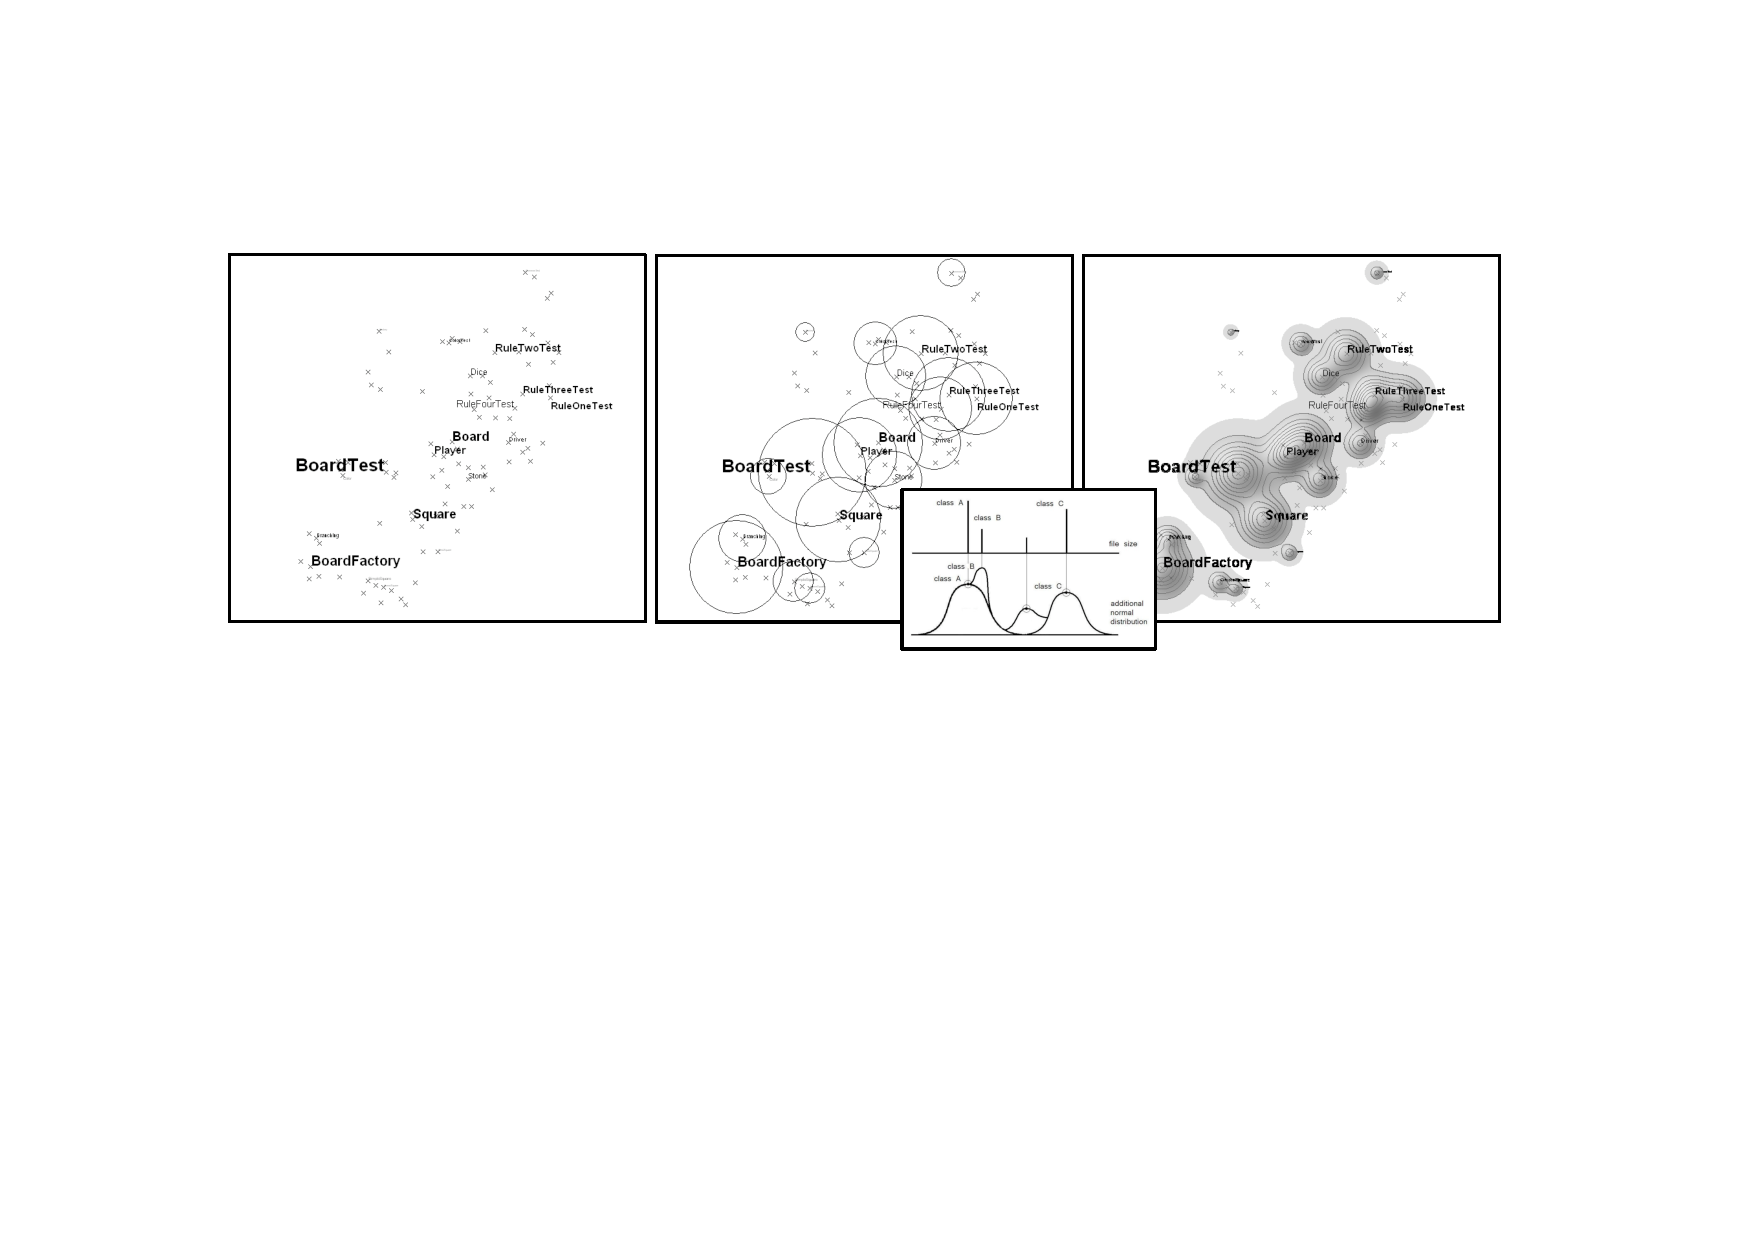
\includegraphics[width=\linewidth]{fig/intro-pipeline}
\end{center}
    \caption{\emph{Construction steps of a software map, from left to right: 1) 2-dimensional embedding of files on the visualization pane; 2.a) circles around each file's location, based on class size in KLOC; 2.b) each file contributes a Gaussian shaped basis function to the elevation model according to its KLOC size; the contributions of all files are summed up; 3) fully rendered map with hill-shading, contour lines, and filename labels.}}
    \label{fig/intro-pipeline}
\end{figure*}

\begin{figure}
\begin{center}
  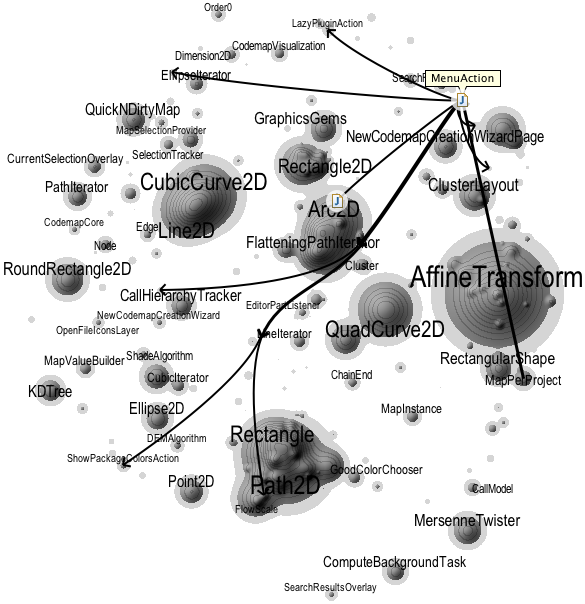
\includegraphics[width=\linewidth]{fig/intro-codemap-example}
\end{center}
    \caption{\emph{Thematic codemap of a software system, here the \Codemap tool itself is shown. Arrow edges show outgoing calls from the {\tt \#getSettingOrDefault} method in the {\tt MenuAction} class, which is currently active in the editor and thus marked with a speech-balloon label.}}
    \label{fig/intro-codemap-example}
\end{figure}

The general approach of \SOCA, as illustrated in \autoref{fig/intro-pipeline}, is as follows:
\begin{enumerate}
\item We parse the vocabulary of source files into term-frequency histograms. All text found in raw source code is taken into account, including not only identifiers but also comments and literals.
\item We use \MDS (MDS) \cite{Borg05a} to map the term-frequency histograms onto the 2D visualization pane. This preserves the lexical co-relation of source files as well as possible.
\item We use cartographic visualization techniques to render an aesthetically appealing landscape.
\end{enumerate}

We implemented the approach in \Codemap, a prototype plug-in for \eclipse that is available under an open-source license. The most recent version\footnote{\url{http://scg.unibe.ch/codemap}} of the plug-in supports the following tasks:


\begin{itemize}
\item Navigation within a software system, be it for development or analysis. \Codemap is integrated with the package explorer and editor of \eclipse. The selection in the package explorer and the selection on the map are linked. Open files are marked with an icon on the map. Double clicking on the map opens the closest file in the editor. When using heat map mode, recently visited classes are highlighted on the map.

\item Comparing software metrics to each other, \eg to compare bug density with code coverage. The map displays search results, compiler errors, and (given the Eclemma plug-in is installed) test coverage information. More information can be added through an plug-in extension point.

\item Social awareness of collaboration in the development team. \Codemap can connect two or more \eclipse instances to show open files of other developers. Colored icons are used to show the currently open files of all developers. Icons are colored by user and updated in real time.

\item Understand a software system's domain. The layout of \Codemap is based on clustering software by topic~\cite{Kuhn07a}, as it has been shown that, over time, the lexicon of source code is more stable than its structure~\cite{Anto07a}. Labels on the map are not limited to class names, but include automatically retrieved keywords and topics.


\item Exploring a system during reverse engineering. \Codemap is integrated with \eclipse's structural navigation features, such as search for callers, implementers, and references. Arrows are shown for search results. We apply the \textsc{Flow Map} algorithm \cite{Phan05a} to  avoid visual clutter by merging parallel arrow edges. \autoref{fig/intro-codemap-example} shows the result of searching for calls to the {\tt \#getSettingOrDefault} method in the {\tt MenuAction} class.
\end{itemize}

%%%%%%%%%% Section 1.5
%%%%%%%%%%
%%%%%%%%%%
%%%%%%%%%%
%%%%%%%%%%
%%%%%%%%%%

\section{Outline}

The dissertation is structured as follows

\begin{description}
% --> related.tex
\item[\autoref{the chapter on related work}] discusses related work. We present various user studies and solutions to code orientation and analyse the shortcomings in the context of each orientation clue.
% --> include.tex
\item[\autoref{the chapter on the MSR user study}] presents a user study that looks at how developers find answers to technical questions and discusses code orientation by cognitive clues.
\item[\autoref{the chapter on hapax}] presents an approach for clustering and summarizing of software systems using lexical information found in source code. The approach is implemented in the \textsc{Hapax} tool. 
\item[\autoref{the chapter on LogLR}] presents an approach that uses lexical information found in source code to summarize parts of a system, the whole system, or even the system's entire evolution. The approach is implemented in the \textsc{EvoClouds} tool.
% --> codemap.tex
\item[\autoref{the chapter on codemap}] introduces \emph{Software Cartography}, an approach to establish a cartographic visualization that facilitates spatial code orientation by individuals or teams. The approach is implemented in the \textsc{Codemap} tool.
\item[\autoref{the chapter on the codemap user study}] reports on a qualitative user study that evaluates the prototype implementation of the Software Cartography approach presented above.
% --> fluff.tex
\item[\autoref{the chapter on chronia}] presents an approach for addressing the episodic memory of developers by providing them with a visualization that tells the story of the team collaboration as recorded by the version control system. The approach is implemented in the \textsc{Chronia} tool.
\item[\autoref{the chapter on bug reports}] presents an approach that uses lexical information found in contributions that developers shared with open source systems to build a recommendation model for bug reports. The approach is implemented  in the \textsc{Devlect} tool.
\item[\autoref{the chapter on codesearch}] presents an approach that uses cross-project collaboration of developers in open source projects to estimate the credibility of code search results. The approach is implemented in the \textsc{Bender} tool.
\item[\autoref{the conclusion}] concludes the dissertation and outlines future work.
\end{description}


%%%%%%%%%%%%

%Also there is a difference in finding code and finding functionality, like if a developer has never seen some piece of source code it is maybe easier to recall the person that has told him about it rather than recalling the source code's name. And just the same with the forward reaching tasks, where often copy-pasting an example is preferred over learning for pragmatic cost considerations.

%- Maybe you recall the song that played on the webradio, so you look that up ...
%- You can use one kind of information as a proxy for other information, so you can you use social and temporal information as a proxy for dependency information (like Tom Zimmermanns work on recommending other locations to update).
%- Photographic memory.
%- The clues have to be turned into actions.
%- How many (inter)actions do you have to do to follow up one clue.
%- Non-conventional questions that people ask themselves but had no tool to answer them before.
%- Two hard problems in CS, caching and naming.

%- JExample generates 'Examples that are worth to be found' .. JExample makes exampels more relevant and more applicable ...
%- Erwann: information can come right from the source code (lexical clues) and can come from somebody else (social clues) from temporal memory or version control system (temporal ones) ...
%- Clues are not about the sources of information, but about the way developers navigate about how they cognitively work when they follow.

%- Change on database propagates to business layer, UI layer ... you know where do go spatially, the space is given by space of software, in other case the space is given by layout of IDE, or given by storage format or persistence format, you know it is there in that text file or on that folder, or in smalltalk open in that window.
%- Codemap: if you observe which clues devs use to refer to code, you'll find all four, but if you look at tool support, you find lexical supported by tools, and temporal only in external tools, and social clues are also not supported, you gonna recall the name of person (ie using the lexical clue of the name as a proxy for the social connection) and spatial is not supported at all, we got the IDE layouted without care about spatial thinking ... code bubbles, code map, and code canvas are about the first systems to take care of this ... 
%- If you ask people to draw maps of their software systems ... as Grady Booch does ... and they always draw an architecture with spatial structural ... so the spatial structure is in their thinking but not in the IDE and even not in the software ...
%- So this why codemap is so interesting because it takes the lexical information and give it a spatial structure in the hope to fill the gap when devs are stuck with lexical clues or social/temporal
%- Spatial clues "somewhere at the end of this file"
%- Structural and spatial is often perceived in the same way, developers tend to use spatial terminology to refer to layers and architectural components.
% - To create a space of software that is visualized on screen, so that people can start using that one to navigate in source code.
%- Erwann: the mental model part?
%- To provide them with a space that will become / should reflect their spatial model...
%- Erwann: if the notion of mental model can be used for all clues ... the other tools gravitate around this spatial mental model.
	
%- All these tools help you to follow up, some more complex clues and unconventional information. It is not that any of these tools addresses a very specific task? Erwann thinks yes it does.
%- I want to help developers, working with code, in particular wrt navigation and understanding, and learning about code.  These clues can be  (ii)  or (iii) it could be temporal or episodic, having a memory from the past that could lead you to an answer, that you've seen it last year (or recall the song that played on the radio) or (iv) 
%- maybe in some years we can add here location based clues, like I've written that code on the train. And in the source of JUnit Kent Beck found it so cool that he added "was written on H�tte at 1200 mUm"
%- and sometime people follow up some very underdeveloped spatial clues. So we know they follow up these clues so we need better tool support and not have to be force to use lexical proxies, you should not be forced to recall the name, but be able to directly work social information when following up a social clues.
%- With spatial information we have this even more special situation that we possible first have to create a space for space.
%- Is there one space to rule them all? or different spaces for different tasks. Codemap that provides one space but still have IDE so onscreen is split, Codecanvas does the same but put the source code on it such that the space become the only onscreen space, the space should be contextually created.
%- The thesis emerged from my work, is that in order to support developers with code navigation we need to build better tools that address the cognitive clues that are used by developers, in particular (in addition to lexical clues) to support navigation by social clues by temporal clues and by spatial clues, and since software has no ...
%- lexical clues are present as identifier names and in comments, social clues are also there we know how has written software and mailinglists etc so people are also there as entity, and also temporal information is tere we have versioning systems that make snapshots of a system in time, but spatial is more difficult ...
%- it somehow maps to the structure of software, which you can extract from source code, but very often spatial is more on a conceptual level and people even use spatial terms on the very level of the arrangement of the UI on screen. So we have three spatial dimensions, structural, conceptual and on screen. So the spatial clues have the least support, so we gotta create a space of software of onscreen to support spatial navigation by developers. 
%- Since software lacks we need to create a spatial view to address the on-screen spatial clues. To create a cartographic representation of other non-spatial properties of the system (like temporal, social and lexical ones) and give them a spatial representation os people can use this forth kind of navigation clues that are actually used. When you talk with developers how they find answers to technical questions related to source code they will tell you sometime they recall a method is at the end of this file, which is onscreen spatial representation. Lemme browser the packages it us up there, down there. And they will use this in the same sentence as some spatial representation that is related to package structure. We have to fix this also up there in the business layer, it as down there in this file, we have to fix this up there it is down there in this file. 
%- Information retrieval to make more interesting things with lexical clues.
%- Evoclouds combine lexical with temporal information.
%- Work by Dominique Matter where we go and mine all the date from the temporal repository and mine the the vocabulary from the contribution of the developers, so we have a new tool that models the expertise of the developers so that now when you have a bug report the system can recommend to you the person. You can turn now a fuzzy textual clue into a social thing.
%- So we asses the credibility of search results solely based on the social network of the authors. This is the way developers have been found to asses the trustworthiness of code, since when you copy code from the internet you do so because you do not want to make the effort of technically understanding it so you look at its author's credibility to make an assessment of trustworthiness.
%- So we have the Chronia tool that has a timeline of the project, and you have a timeline of each file and you see the collaboration patterns. When you show this to developers the go crazy, with this visualization the episodic memory is brought back. You can learn about team members.


